
% Copyright (c) 2015 - 2019 Mario Mlačak, mmlacak@gmail.com
% Published as Public Domain work, under CC0 1.0 Universal Public Domain Dedication. See LICENSING, COPYING files for details.

% Classical Chess -----------------------------------------------------
\chapter*{Classical Chess}
\addcontentsline{toc}{chapter}{Classical Chess}
\label{ch:Classical Chess}

\begin{flushright}
\parbox{0.8\textwidth}{
\emph{A great war leaves the country with three armies -
an army of cripples, an army of mourners, and an army of thieves. \newline
\hspace*{\fill}{\textperiodcentered \textperiodcentered \textperiodcentered \hspace*{0.2em} German proverb} } }
\end{flushright}

\noindent
About Classical Chess is written really everything already, and I have
nothing to add, except to use it as an example on how to read the book.

\clearpage % ..........................................................
% Pieces **************************************************************

\section*{Pieces}
\addcontentsline{toc}{section}{Pieces}
\label{sec:Classical Chess/Pieces}

The easiest way to introduce readers to the rendering of classical pieces
is to show chessboard with initial setup:

\noindent
\begin{figure}[!h]
\includegraphics[width=1.0\textwidth, keepaspectratio=true]{boards/02_classical.png}
\caption{Classical Chess, initial setup}
\label{fig:02_classical}
\end{figure}

\noindent
You can compare this with official rendering at \algfmt{FIDE~2.3}.

\clearpage % ..........................................................

\subsection*{Bishop}
\addcontentsline{toc}{subsection}{Bishop}
\label{sec:Classical Chess/Pieces/Bishop}

\noindent
\begin{wrapfigure}[12]{l}{0.4\textwidth}
\centering
\includegraphics[width=0.4\textwidth, keepaspectratio=true]{pieces/bishop/02_classical.png}
\caption{Bishop}
\label{fig:bishop/02_classical}
\end{wrapfigure}
New pieces are introduced with zoomed-in image, on a \mbox{2 $\times$ 2} board.
Light pieces are rendered on a lower row, dark pieces are on an upper row,
regardless of actual colors used in a particular variant. \newline
\indent
Light fields are always in lower-right and upper-left corner, while dark fields
are always in lower-left and upper-right corner, regardless which actual colors
are used to paint board.

% ************************************************************** Pieces
% \clearpage % ..........................................................
% Chessboard **********************************************************

\section*{Chessboard}
\addcontentsline{toc}{section}{Chessboard}
\label{sec:Classical Chess/Chessboard}

As seen on the chessboard on previous page, light player starts from bottom of
a chessboard, while dark player starts from top. This arrangement is used by FIDE
(see \algfmt{FIDE~2.3}), and also in this book for all examples and for all new
variants, regardless the size of a chessboard used in a variant.

In such a setup, color of lower-right (and upper-left) corner are determined by
FIDE to be light colored, see \algfmt{FIDE~2.1}; this also applies to all new
variants, regardless which actual colors are used to paint chessboards.

\clearpage % ..........................................................
% Examples ============================================================

\subsection*{Examples}
\addcontentsline{toc}{subsection}{Examples}
\label{sec:Classical Chess/Chessboard/Examples}

\vspace*{-0.7\baselineskip}
\noindent
\begin{figure}[!h]
\includegraphics[width=1.0\textwidth, keepaspectratio=true]{examples/02_c/scn_cc_01_bishop_not_blocked.png}
% \vspace*{-1.4\baselineskip}
\caption{Bishop not blocked}
\label{fig:scn_cc_01_bishop_not_blocked}
\end{figure}

. . .

\clearpage % ..........................................................

\vspace*{-2.1\baselineskip}
\noindent
\begin{figure}[!h]
\includegraphics[width=1.0\textwidth, keepaspectratio=true]{examples/02_c/scn_cc_02_bishop_blocked.png}
% \vspace*{-1.4\baselineskip}
\caption{Bishop blocked}
\label{fig:scn_cc_02_bishop_blocked}
\end{figure}

. . .

% ============================================================ Examples
% ********************************************************** Chessboard
\clearpage % ..........................................................

\noindent
\TODO :: introduction \newline

\noindent
\textrightarrow basic terminology: turn, move, cycle, figure, ... \newline
\textrightarrow new terminology: rush, steps, step-fields, capture-fields \newline
\textrightarrow conflicting terminology: activating a piece, ply (?) \newline

\noindent
\textrightarrow arrows \& colors \newline
\textrightarrow markers, texts (enumerations vs. labels) \newline
\textrightarrow navigation \newline

\noindent
\textrightarrow context, exceptions \newline

\clearpage % ..........................................................
% ----------------------------------------------------- Classical Chess
